% !TeX root = Thesis.tex

\begin{figure}[ht]
    \centering
    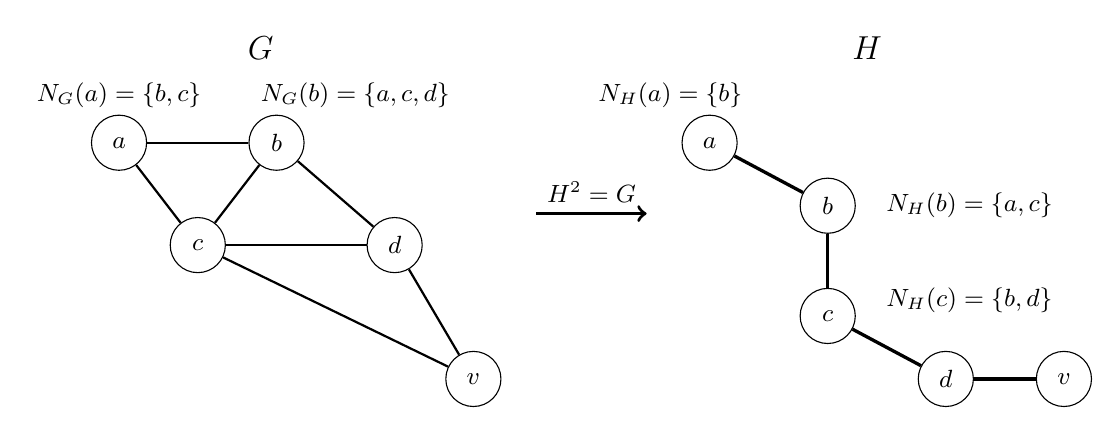
\begin{tikzpicture}[
        vertex/.style={
            circle,
            draw,
            fill=white,
            minimum size=7mm,
            inner sep=0pt
        },
        Gedge/.style={thick},
        Hedge/.style={very thick},
        every node/.style={font=\small}
    ]

    \node at (1.8,4.2) {\large $G$};

    \node[vertex] (aG) at (0,3) {$a$};
    \node[vertex] (bG) at (2,3) {$b$};
    \node[vertex] (cG) at (1,1.7) {$c$};
    \node[vertex] (dG) at (3.5,1.7) {$d$};
    \node[vertex] (vG) at (4.5,0) {$v$};

    \draw[Gedge] (aG)--(bG);
    \draw[Gedge] (aG)--(cG);
    \draw[Gedge] (bG)--(cG);
    \draw[Gedge] (bG)--(dG);
    \draw[Gedge] (cG)--(dG);
    \draw[Gedge] (cG)--(vG);
    \draw[Gedge] (dG)--(vG);

    \node[align=center] at (0,3.6)
        {$N_G(a)=\{b,c\}$};

    \node[align=center] at (3.0,3.6)
        {$N_G(b)=\{a,c,d\}$};

    \draw[->, very thick] (5.3,2.1)--(6.7,2.1)
        node[midway, above] {$H^2=G$};

    \node at (9.5,4.2) {\large $H$};

    \node[vertex] (aH) at (7.5,3) {$a$};
    \node[vertex] (bH) at (9,2.2) {$b$};
    \node[vertex] (cH) at (9,0.8) {$c$};
    \node[vertex] (dH) at (10.5,0) {$d$};
    \node[vertex] (vH) at (12,0) {$v$};

    \draw[Hedge] (aH)--(bH);
    \draw[Hedge] (bH)--(cH);
    \draw[Hedge] (cH)--(dH);
    \draw[Hedge] (dH)--(vH);

    \node[align=left] at (7.0,3.6)
        {$N_H(a)=\{b\}$};

    \node[align=left] at (10.8,2.2)
        {$N_H(b)=\{a,c\}$};

    \node[align=left] at (10.8,1.0)
        {$N_H(c)=\{b,d\}$};

    \end{tikzpicture}
    \caption{The forced local structure in the Tail Lemma. The square root
    $H$ contains the path $a-b-c-d$. Consequently, $ac,bd\in E_G$ as
    distance-two edges. For an external neighbour $v$ of $c$, the Tail
    Lemma gives $dv\in E_H$, and hence $dv\in E_G$.}
    \label{fig:tail-lemma}
\end{figure}